\documentclass{article}
\usepackage{amsfonts, amsthm, amsmath, amssymb, mathtools, ulem, mathrsfs, physics, esint, siunitx, tikz-cd}
\usepackage{pdfpages, fullpage, color, microtype, cancel, textcomp, markdown, hyperref, graphicx}
\usepackage{enumitem}
\usepackage{algorithm}
\usepackage{algpseudocode}
\graphicspath{{./images/}}
\usepackage[english]{babel}
\usepackage[autostyle, english=american]{csquotes}
\MakeOuterQuote{"}
\usepackage{xparse}
\usepackage{tikz}

\usepackage{calligra}
\DeclareMathAlphabet{\mathcalligra}{T1}{calligra}{m}{n}
\DeclareFontShape{T1}{calligra}{m}{n}{<->s*[2.2]callig15}{}
\newcommand{\script}[1]{\ensuremath{\mathcalligra{#1}}}
\newcommand{\scr}{\script r}

% fonts
\def\mbb#1{\mathbb{#1}}
\def\mfk#1{\mathfrak{#1}}
\def\mbf#1{\mathbf{#1}}
\def\tbf#1{\textbf{#1}}

% common bold letters
\def\bP{\mbb{P}}
\def\bC{\mbb{C}}
\def\bH{\mbb{H}}
\def\bI{\mbb{I}}
\def\bR{\mbb{R}}
\def\bQ{\mbb{Q}}
\def\bZ{\mbb{Z}}
\def\bN{\mbb{N}}

% brackets
\newcommand{\br}[1]{\left(#1\right)}
\newcommand{\sbr}[1]{\left[#1\right]}
\newcommand{\brc}[1]{\left\{#1\right\}}
\newcommand{\lbr}[1]{\left\langle#1\right\rangle}

% vectors
\renewcommand{\i}{\hat{\imath}}
\renewcommand{\j}{\hat{\jmath}}
\renewcommand{\k}{\hat{k}}
\newcommand{\proj}[2]{\text{proj}_{#2}\br{#1}}
\newcommand{\m}[2][b]{\begin{#1matrix}#2\end{#1matrix}}
\newcommand{\arr}[3][\sbr]{#1{\begin{array}{#2}#3\end{array}}}

% misc
\NewDocumentCommand{\seq}{O{n} O{1} O{\infty} m}{\br{#4}_{{#1}={#2}}^{#3}}
\NewDocumentCommand{\app}{O{x} O{\infty}}{\xrightarrow{#1\to#2}}
\newcommand{\sm}{\setminus}
\newcommand{\sse}{\subseteq}
\renewcommand{\ss}{\subset}
\newcommand{\vn}{\varnothing}
\newcommand{\lc}{\epsilon_{ijk}}
\newcommand{\ep}{\epsilon}
\newcommand{\vp}{\varphi}
\renewcommand{\th}{\theta}
\newcommand{\cjg}[1]{\overline{#1}}
\newcommand{\inv}{^{-1}}
\DeclareMathOperator{\im}{im}
\DeclareMathOperator{\id}{id}
\newcommand{\ans}{\tbf{Ans. }}
\newcommand{\pf}{\tbf{Pf. }}
\newcommand{\imp}{\implies}
\newcommand{\impleft}{\reflectbox{$\implies$}}
\newcommand{\ck}{\frac1{4\pi\ep_0}}
\newcommand{\ckb}{4\pi\ep_0}
\newcommand{\sto}{\longrightarrow}
\DeclareMathOperator{\cl}{cl}
\DeclareMathOperator{\intt}{int}
\DeclareMathOperator{\bd}{bd}
\DeclareMathOperator{\Span}{span}
\newcommand{\floor}[1]{\left\lfloor#1\right\rfloor}
\newcommand{\ceil}[1]{\left\lceil#1\right\rceil}
\newcommand{\fxn}[5]{#1:\begin{array}{rcl}#2&\longrightarrow & #3\\[-0.5mm]#4&\longmapsto &#5\end{array}}
\newcommand{\sep}[1][.5cm]{\vspace{#1}}
\DeclareMathOperator{\card}{card}
\renewcommand{\ip}[2]{\lbr{#1,#2}}
\renewcommand{\bar}{\overline}
\DeclareMathOperator{\cis}{cis}
\DeclareMathOperator{\Arg}{Arg}
\DeclareMathOperator{\diag}{diag}

% title
\title{Scientific Computing HW 11}
\author{Ryan Chen}
%\date{\today}
\setlength{\parindent}{0pt}


\begin{document}
	
\maketitle



\tbf{Problem 1.}

\begin{enumerate}[label=(\alph*)]
	
\item The form of solution is
$$u(x,t) = \frac12[\vp(x+at)+\vp(x-at)] + \frac{1}{2a}\int_{x-at}^{x+at}\psi(s)ds$$
First find $u_{tt}$.
$$u_t = \frac12[\vp'(x+at)\cdot a+\vp'(x-at)\cdot(-a)] + \frac{1}{2a}[\psi(x+at)\cdot a-\psi(x-at)\cdot(-a)]$$
$$= \frac{a}{2}[\vp'(x+at)-\vp'(x-at)] + \frac12[\psi(x+at)+\psi(x-at)]$$
$$u_{tt} = \frac{a^2}{2}[\vp''(x+at)+\vp''(x-at)] + \frac a2[\psi'(x+at)-\psi'(x-at)]$$
Then find $a^2u_{xx}$ and see that it equals $u_{tt}$, hence $u$ solves the PDE.
$$u_x = \frac12[\vp'(x+at)+\vp'(x-at)] + \frac{1}{2a}[\psi(x+at)-\psi(x-at)]$$
$$u_{xx} = \frac12[\vp''(x+at)+\vp''(x-at)] + \frac{1}{2a}[\psi'(x+at)-\psi'(x-at)]$$
$$a^2u_{xx} = \frac{a^2}{2}[\vp''(x+at)+\vp''(x-at)] + \frac{a}{2}[\psi'(x+at)-\psi'(x-at)] = u_{tt}$$


\item The form of solution is
$$u(x,t) = \frac12[\vp(x+at)+\vp(x-at)] + \frac{1}{2a}\int_{x-at}^{x+at}\psi(s)ds$$
From its terms we see that $u(x,t)$ depends precisely on the values of $\vp$ at $x\pm at$ and the values of $\psi$ on $[x-at,x+at]$. Thus the domain of dependence of a point $(x,t)$ is $\brc{(s,0):x-at\le s\le x+at}$.


\item We see that
$$w := \m{u_t \\ u_x}
\imp w_x = \m{u_{tx} \\ u_{xx}}$$
so that
$$w_t = \m{u_{tt} \\ u_{xt}}
= \m{0u_{tx}+a^2u_{xx} \\ 1u_{tx}+0u_{xx}}
= \underbrace{\m{0 & a^2 \\ 1 & 0}}_{=:A}\m{u_{tx} \\ u_{xx}}
= Aw_x$$
Then
$$u_x\eval_{t=0} = \frac12[\vp'(x)+\vp'(x)] + \frac{1}{2a}[\psi(x)-\psi(x)]
= \vp'(x)$$
so that the initial condition for $w$ is
$$w\eval_{t=0} = \m{u_t\eval_{t=0} \\ u_x\eval_{t=0}}
= \m{\psi(x) \\ \vp'(x)}$$


\item The eigenvalues of $A$ are
$$0 = \det(A-\lambda I)
= \m[v]{-\lambda & a^2 \\ 1 & -\lambda}
= \lambda^2 - a^2
= (\lambda-a)(\lambda+a)
\imp \lambda_1 = a,~\lambda_2 = -a$$
Eigenvectors $v_1,v_2$ of $A$ are
$$A-\lambda_1I = \m{-a & a^2 \\ 1 & -a}
\imp v_1 = \m{a \\ 1}$$
$$A-\lambda_2I = \m{a & a^2 \\ 1 & a}
\imp v_2 = \m{-a \\ 1}$$
Diagonalizing $A$,
$$A = C\Lambda C\inv,
\quad C := [v_1,v_2],
\quad \Lambda := \diag(\lambda_1,\lambda_2)$$

Changing variable, we obtain independent PDEs.
$$y := C\inv w = \m{\xi \\ \eta}
\imp w = Cy
\imp w_t = Cy_t,
~w_x = Cy_x$$
$$\imp 0 = w_t - Aw_x
= Cy_t - C\Lambda C\inv Cy_x
= C(y_t-\Lambda y_x)
\imp y_t - \Lambda y_x = 0
\imp y_t = \Lambda y_x$$
$$\imp \xi_t = \lambda_1\xi_x = a\xi_x,
~\eta_t = \lambda_2\eta_x = -a\eta_x$$

First find $C\inv$.
$$\det C = \m[v]{a & -a \\ 1 & 1}
= 2a
\imp C\inv = \frac{1}{2a}\m{1 & a \\ -1 & a}$$
Then we find the initial condition for $y$, i.e. the initial conditions for $\xi,\eta$.
$$\m{\psi(x) \\ \vp'(x)} = w\eval_{t=0} = Cy\eval_{t=0}
\imp y\eval_{t=0} = C\inv\m{\psi(x) \\ \vp'(x)}
= \frac{1}{2a}\m{\psi(x)+a\vp'(x) \\ -\psi(x)+a\vp'(x)}$$


\item Code: \url{github.com/RokettoJanpu/Scientific-Computing-2/blob/main/hw11 q1.ipynb}

Lax--Friedrichs:
\begin{center}
	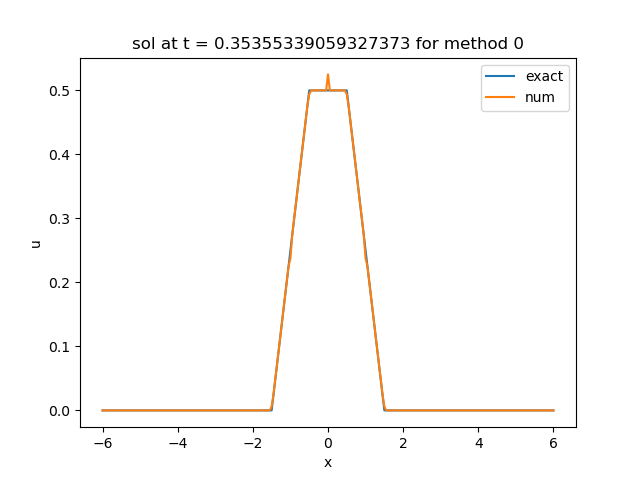
\includegraphics[scale=.4]{hw11 sol n = 10 method 0}
	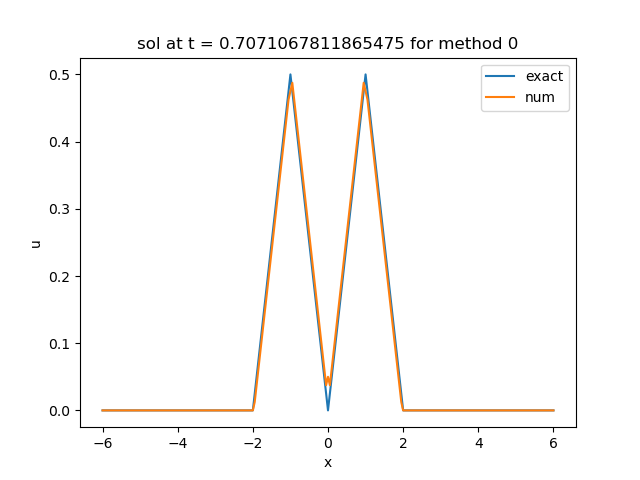
\includegraphics[scale=.4]{hw11 sol n = 20 method 0}
\end{center}
\begin{center}
	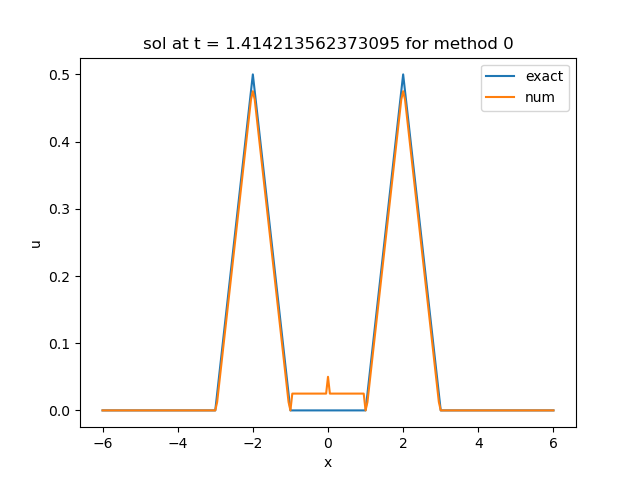
\includegraphics[scale=.4]{hw11 sol n = 40 method 0}
	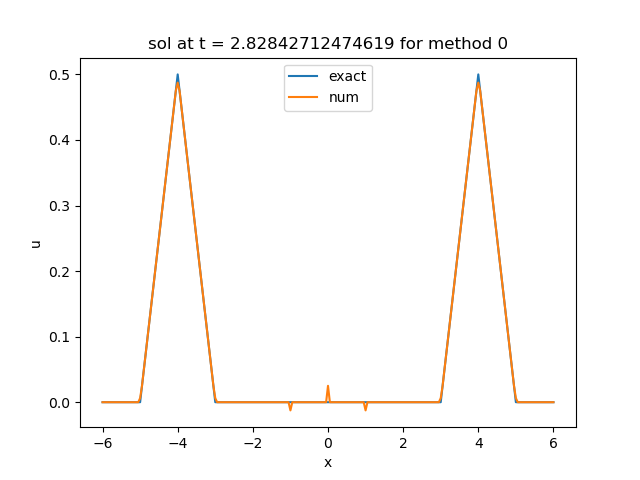
\includegraphics[scale=.4]{hw11 sol n = 80 method 0}
\end{center}

Upwind:
\begin{center}
	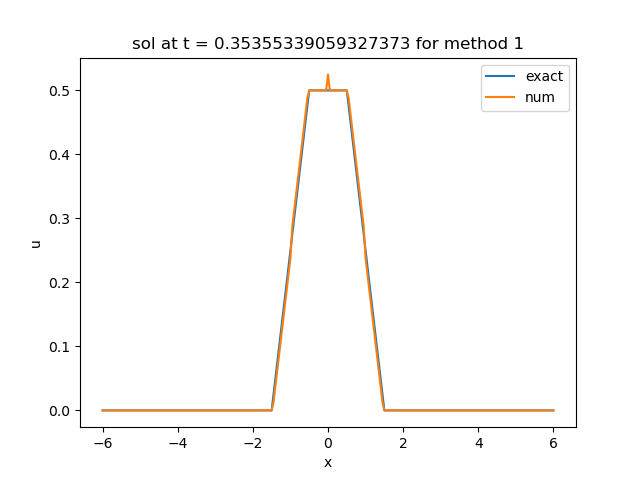
\includegraphics[scale=.4]{hw11 sol n = 10 method 1}
	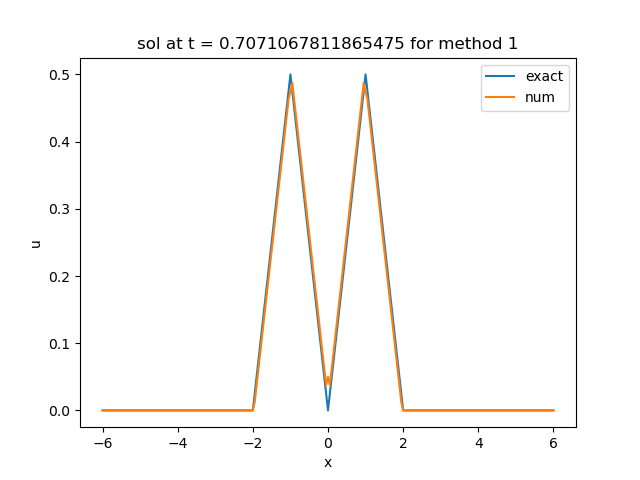
\includegraphics[scale=.4]{hw11 sol n = 20 method 1}
\end{center}
\begin{center}
	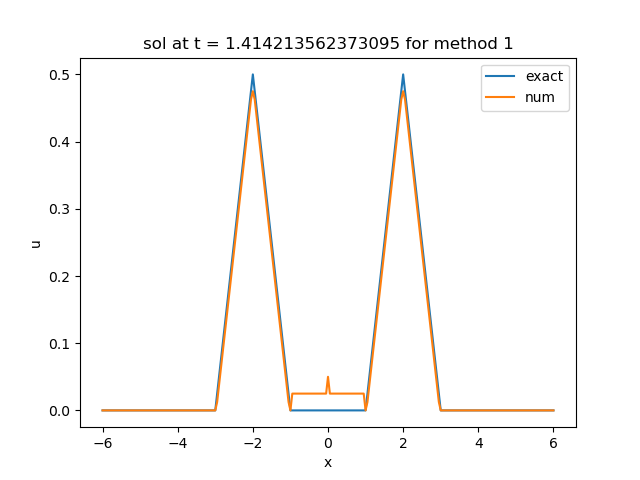
\includegraphics[scale=.4]{hw11 sol n = 40 method 1}
	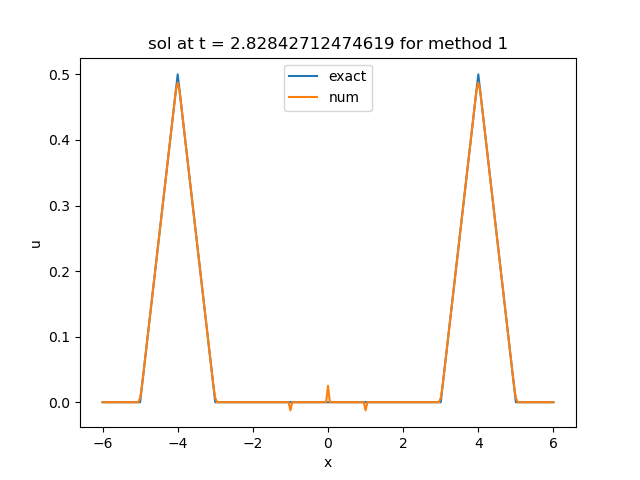
\includegraphics[scale=.4]{hw11 sol n = 80 method 1}
\end{center}

Beam--Warming:
\begin{center}
	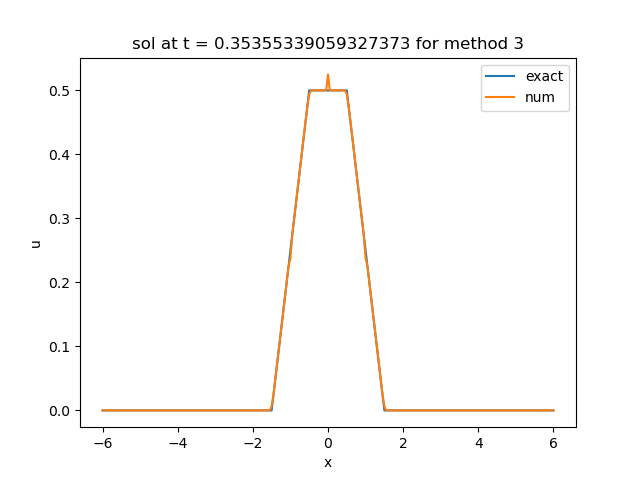
\includegraphics[scale=.4]{hw11 sol n = 10 method 3}
	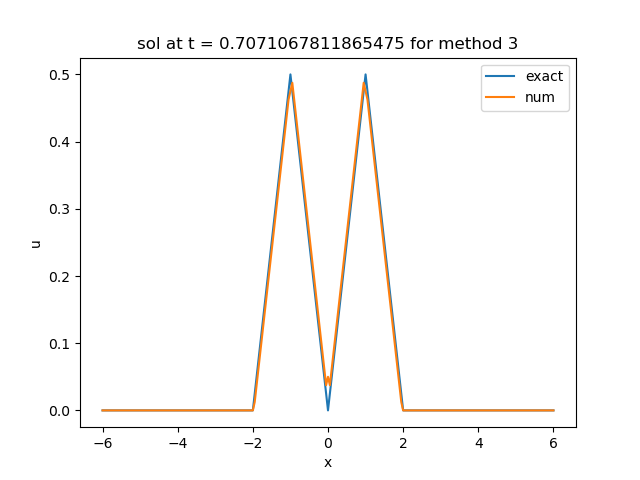
\includegraphics[scale=.4]{hw11 sol n = 20 method 3}
\end{center}
\begin{center}
	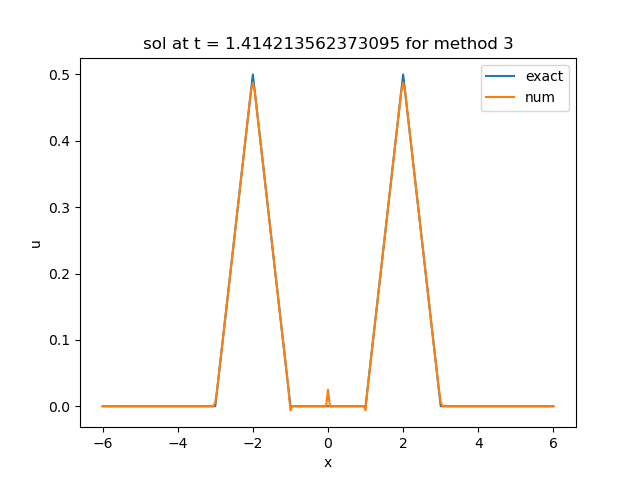
\includegraphics[scale=.4]{hw11 sol n = 40 method 3}
	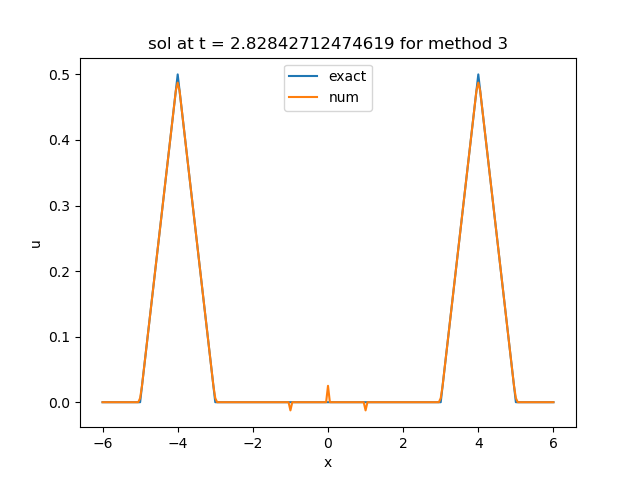
\includegraphics[scale=.4]{hw11 sol n = 80 method 3}
\end{center}
	
\end{enumerate}


	
\end{document}